\chapter{Az S-gráf keretrendszer} \label{S-graph}
Az S-gráf keretrendszer egy irányított gráf modellből, az S-gráfból és a hozzá tartozó algoritmusokból áll \cite{SANMARTI1998S847}. 
Az S-gráf egy speciális irányított gráf, amely nem csupán a probléma vizualizációjára képes, hanem egy matematikai modell is.
A keretrendszerben a recepteket, valamint a félkész-, illetve a teljes ütemterveket is az S-gráf reprezentálja.
Ezekben a gráfokban a termékeket, illetve a feladatokat a csúcsok jelölik, amelyeket csomópontoknak nevezünk.
Ezenkívül, ha két feladat között összeköttetés van, ezt a gráfon a két feladatot reprezentáló csomópontok közötti irányított él jelöli.
Az ütemezési információ nélküli S-gráfot recept gráfnak (\textbf{recipe graph)} nevezzük, melyre egy példa a \ref{recipeGraph}. ábrán látható.
\begin{figure}[H]
\begin{center}
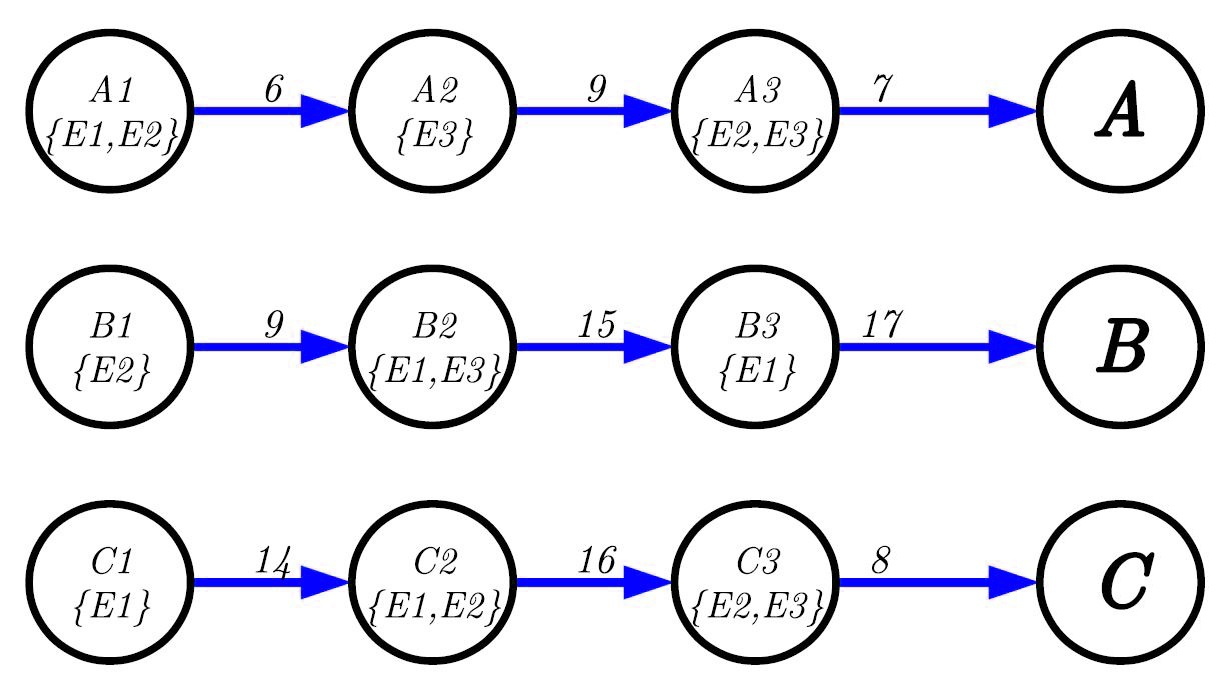
\includegraphics[scale=0.375]{recipeGraph}
\caption{A recept gráf szemléltetése}
\label{recipeGraph}
\end{center}
\end{figure}
Az ábrán látható jobb oldali kettő csomópont (A,B) jelöli a termékeket, a többi csomópont pedig a részfeladatokat, amelyeket el kell végezni a termékek előállítása érdekében.
A recept gráf irányított élei reprezentálják egyrészt két részfeladat közötti függőséget, abban ez esetben például, ha ez egyik részfeladat állítja elő a másik részfeladathoz szükséges bemeneti részterméket, másrészt a részfeladatok és a késztermékek közötti függőséget.
A recept gráf minden részfeladathoz tartozó csomópontjához tartozik egy halmaz, amely azon berendezések nevét tartalmazza, amelyek képesek adott részfeladat megoldására.
Az éleken található súlyok pedig a részfeladat megoldásához szükséges gyártási időt reprezentálják, abban az esetben, ha egy részfeladatot több berendezés is el tud végezni, az irányított él súlya a berendezésekhez tartozó gyártási idők közül a legkisebb lesz.

Az S-gráf keretrendszerben található algoritmusok az előzőekben bemutatott recept gráfot egészítik ki ütemezési élekkel, amelyek az algoritmus által meghozott ütemezési döntéseket reprezentálják.
Az ily módon előállított gráfot, függetlenül attól, hogy van-e még meghozatlan ütemezési döntés, vagy pedig a teljes ütemezés megtörtént, ütemezési gráfnak (\textbf{schedule graph}) nevezzük.
A \ref{recipeGraph}. pontban látható recept gráf alapján előállított egy lehetséges ütemezési gráf a \ref{scheduleGraph}. ábrán látható.
\begin{figure}[H]
\begin{center}
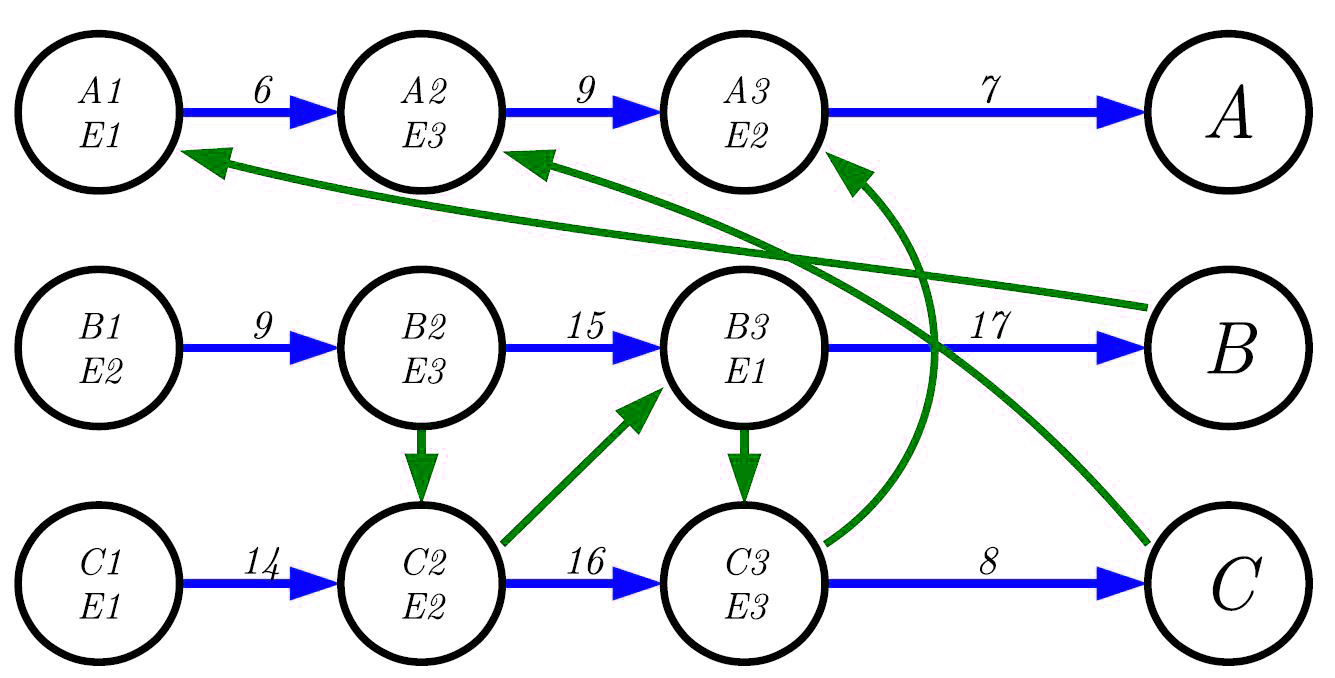
\includegraphics[scale=0.375]{scheduleGraph}
\caption{Az ütemezési gráf szemléltetése}
\label{scheduleGraph}
\end{center}
\end{figure}
Az ábrán látható gráfon már minden ütemezési döntés meghozásra került, a zöld élek modellezik az ütemező algoritmus által meghozott ütemezési döntéseket.
A részfeladatokat reprezentáló csomópontokon immáron a lehetséges berendezések halmaza helyett egy konkrét berendezés jelölése található, amely az adott részfeladat elvégzésére hivatott az adott ütemterv szerint.
Az ütemezési élek súlya alapértelmezetten $0$, ha az adott problémában nem számolunk például részfeladatok közötti szállítási-, átállási-, illetve tisztítási időkkel.
Az adott berendezéshez rendelt részfeladatok sorrendje könnyen leolvasható az ütemezési gráfról, erre egy példa a \ref{unitSequence}. ábrán látható.
\begin{figure}[H]
\begin{center}
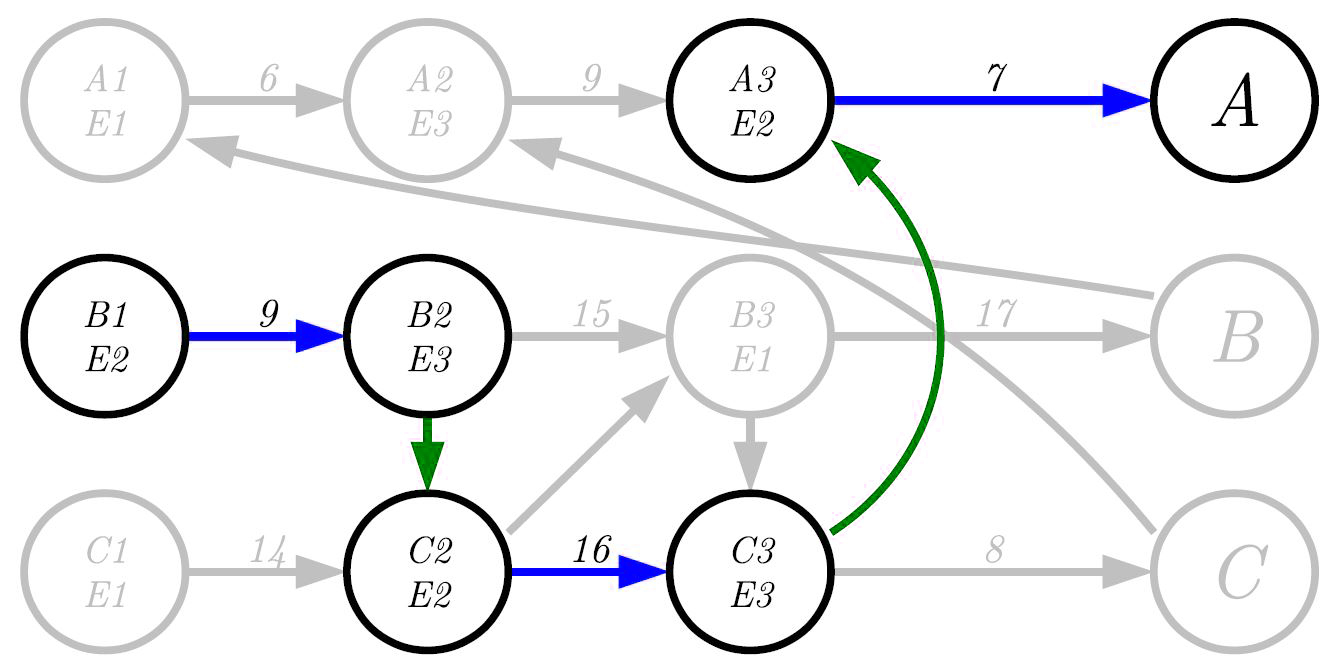
\includegraphics[scale=0.375]{unitSequence}
\caption{Az E1 berendezéshez rendelt részfeladatok sorrendje}
\label{unitSequence}
\end{center}
\end{figure}
Az ábra alapján leolvasható, hogy az E1 berendezés először a B1 részfeladatot végzi el, majd a A1, azután pedig az A2 fog következni.
Az ábrán megfigyelhető továbbá az is, hogy a zöld ütemezési nyíl nem közvetlenül a B1 csomópontból, hanem a B2-ből került behúzásra az A1 felé.
Ezen jelölés azt szemlélteti, hogy A1 feladat elkezdéséhez nem elegendő az, hogy E1 berendezés elvégezze B1 feladatot, de a B1 feladat során termelt részterméket E2-nek először át kell vennie E1 berendezéstől, addig ugyanis az E1 berendezésben kerül tárolásra NIS tárolási irányelv szerint.

\section{Makespan minimalizálás az S-gráf keretrendszerben}
Az S-gráf keretrendszer eredetileg makespan minimalizációs célokra lett megalkotva.
A makespan minimalizáló algoritmus egy Branch \& Bound algoritmus, melynek segítségével adott receptgráffal reprezentált termékek gyártási ideje minimalizálható.
Az algoritmus fontos szerepet játszik azonban a \ref{SgraphProfitMax}. alfejezetben tárgyalt throughput maximalizáló algoritmusban is, éppen ezért az algoritmus rövid áttekintése hasznos lehet a továbbiakban, ezt tartalmazza jelen alfejezet.
Az S-gráf keretrendszer makespan minimalizáló algoritmusának lefutására egy részletes példa megtalálható a CD melléklet \fileName{Algoritmusok} mappájában \fileName{DO\_Sgraph\_Makespan\_Minimization.odg} néven. 
Az algoritmus először végtelenre állítja be a makespan értékét, valamint inicializálja a nyitott részproblémák halmazát, amelyben kezdetben csupán a recept gráf található.
Minden iteráció során egy részprobléma kerül kiválasztásra ebből a halmazból, ez a kiválasztás többféle stratégia alapján történhet, ezért ennek mikéntje implementáció függő.
Az iteráció kezdetén a  részprobléma kiértékelésre kerül egy bound függvény által abból a szempontból, hogy optimális eredményt képes-e szolgáltatni.
Ez a bound függvény leggyakrabban a gráfban található leghosszabb út alapján kerül kiszámításra.
Ha az aktuális részprobléma bound értéke nem kisebb mint az aktuális legjobb eredmény, az iteráció véget ér, egy új részprobléma kerül kiválasztásra a halmazból.
Ha a bound érték kisebb mint az aktuális legjobb érték, az algoritmus leellenőrzi, hogy a részprobléma esetén minden ütemezési döntés meghozásra került-e.
Ha ez a feltétel igaz, akkor a makespan értéke frissítésre kerül az aktuális részprobléma bound-jával, valamint elmentésre kerül az ütemezési gráf is, mint az eddigi legjobb megoldás.
Abban az esetben, ha a részproblémához tartozó ütemezési gráf nem teljes, az algoritmus az elérhető berendezésekhez rendeli a még elérhető feladatokat.
Minden berendezéshez rendelt feladat esetén lemásolásra kerül az aktuális ütemezési gráf.
Ezen másolatok kiegészítésre kerülnek a hozzárendelés alapján behúzható ütemezési élekkel, valamint ezen élek súlyaival.
Ezután minden ilyen módon létrehozott új gráf hozzáadásra kerül a nyitott részproblémák halmazához.
Az algoritmus akkor ér véget, ha ez a halmaz kiürül, ebben az esetben visszaadásra kerül a legjobb megoldást reprezentáló ütemezési gráf és a hozzá tartozó makespan érték, ha létezik a problémának legalább egy feasible megoldása. 
\section{Profit maximalizálás az S-gráf keretrendszerrel} \label{SgraphProfitMax}
A makespan minimalizáláson kívül az S-gráf keretrendszer később kibővítésre került egy throughput maximalizáló algoritmussal, amely segítségével immáron throughput maximalizálásra is képes.
Az throughput maximalizáló algoritmus alapötletét Majozi és Friedler \cite{doi:10.1021ie0604472}, valamint Holczinger és társai \cite{HOLCZINGER2007649} fektették le.
Az algoritmus lényege, hogy a termékek lehetséges batch darabszámai alapján különböző konfigurációk kerülnek létrehozásra, melyek között az algoritmus segítségével eredményül kapható a legnagyobb throughputot eredményező konfiguráció, ha létezik megvalósítható (feasible) megoldás a problémára.
Egy konfiguráció alatt tehát azt értjük, hogy adott termékből hány batch-et termelünk.
Ezen konfigurációk elképzelhetőek egy $n$ dimenziós térben, ahol $n$ a különböző termékek számát jelöli.
Ebben a térben a tengelyek menti megoldások azokat az eseteket jelölik, melyekben csak egy fajta terméket termelünk.
A throughput maximalizáló algoritmus működésének egy példán keresztül történő szemléltetésére készült folyamatábra a CD melléklet \fileName{Algoritmusok} mappájában található \fileName{DO\_Sgraph\_Throughput\_Maximization.odp} néven.
Ezen fájl alapján a fentiekre példa két termék esetén a következő koordináta rendszer:
 \begin{figure}[H]
\begin{center}
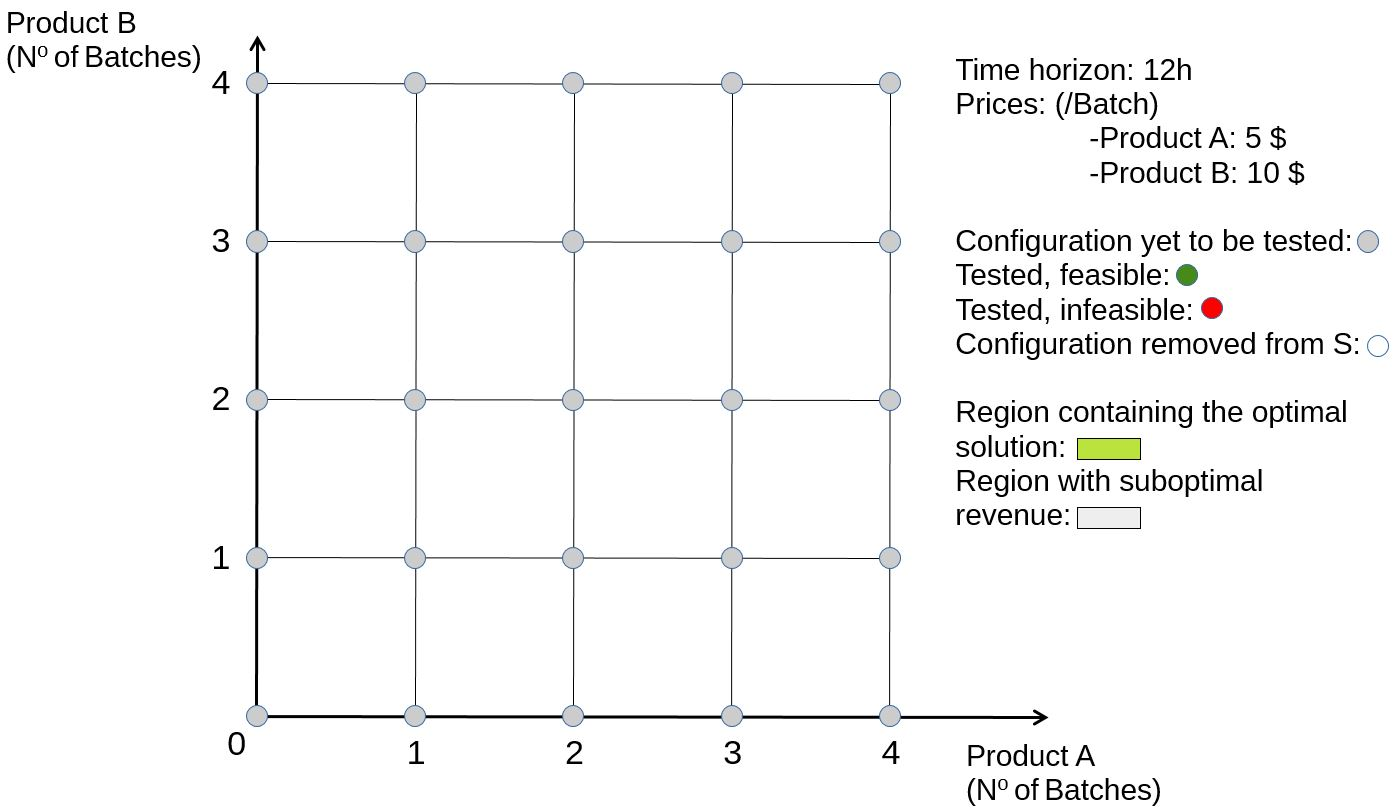
\includegraphics[scale=0.4]{throughputCoordinate}
\caption{A konfigurációkat tartalmazó tér szemléltetése két termék esetén}
\label{throughputCoordinate}
\end{center}
\end{figure}
Kezdetben a konfigurációk halmaza tartalmazza az összes lehetséges konfigurációt az adott termékekre, majd minden iteráció során kiválasztásra kerül egy konfiguráció, amelynek teszteljük feasible-itását, azaz hogy a rendelkezésre álló időhorizont alatt megvalósítható-e adott konfiguráció legyártása.
Ennek tesztelése a korábban már említett makespan minimalizáló algoritmus felhasználásával a legegyszerűbb.
A makespan minimalizáló algoritmusnak átadásra kerül adott konfiguráció recept gráfja, majd az eredményül kapott idő érték összehasonlításra kerül a rendelkezésre álló időhorizonttal, ha a kapott érték nagyobb annál, az adott konfiguráció nem valósítható meg (infeasible). 
Ha az adott konfiguráció megvalósítható a rendelkezésre álló időhorizont alatt, kiszámításra kerül az adott konfiguráció által nyújtott profit, ha ez nagyobb az eddigi legjobb értéknél, frissíteni kell a legjobb értéket adott konfiguráció revenue értékével.
Kezdetben a tengelyek menti konfigurációk kerülnek tesztelésre mind addig, még az összes tengelyen el nem jutunk az első megvalósíthatatlan (infeasible) konfigurációig.
Ezzel előáll egy tér, amely tartalmazza az optimális megoldást, amelyet már csak meg kell találni.
Ennek szemléltetésére szolgál a \ref{optSolRegion}.  ábra.
 \begin{figure}[H]
\begin{center}
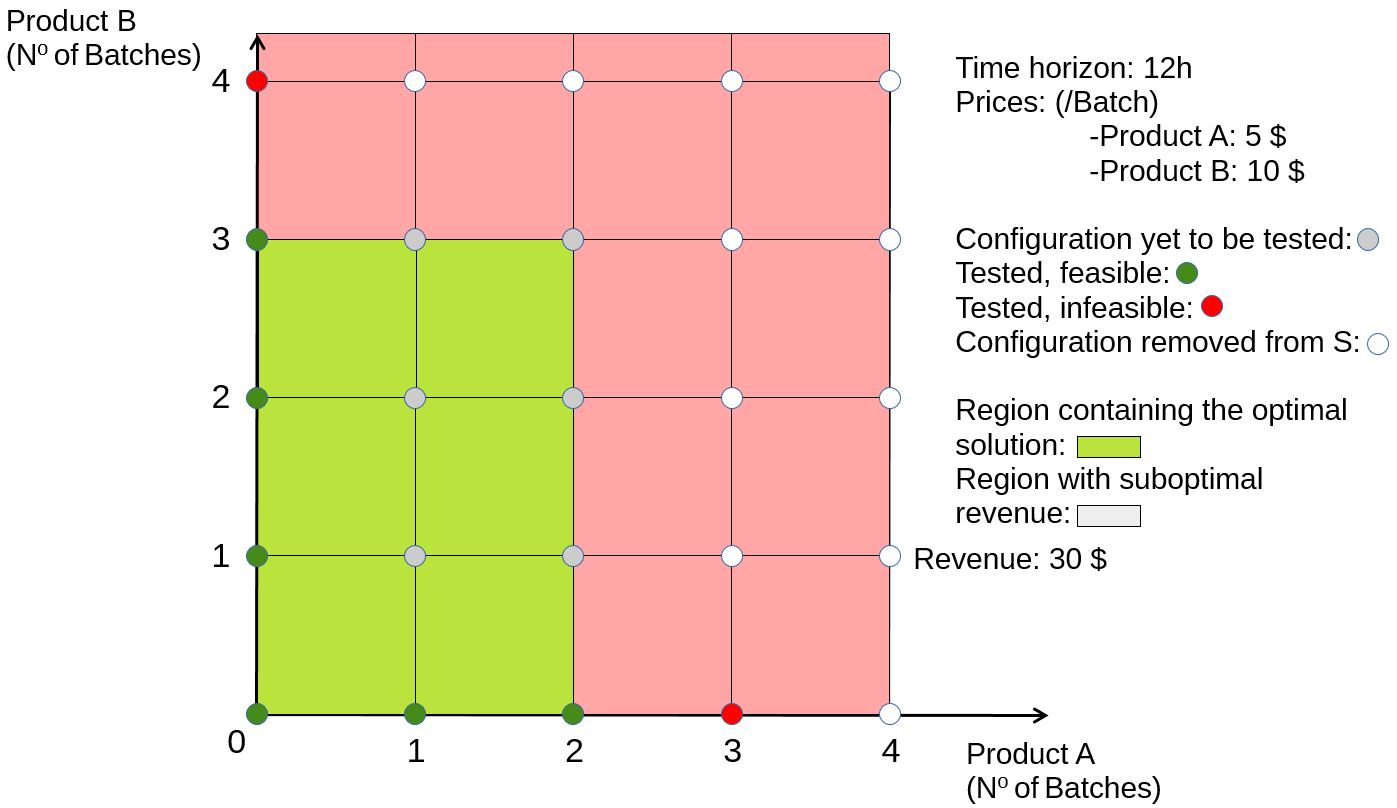
\includegraphics[scale=0.4]{optSolRegion}
\caption{Példa az optimális megoldást tartalmazó térre két termék esetén}
\label{optSolRegion}
\end{center}
\end{figure}
Mivel a konfigurációk tesztelése erőforrás igényes feladat, ezért a konfigurációk kiválasztásának sorrendje ezen a téren belül nem mindegy, többféle stratégia létezik az algoritmus gyorsítására \cite{phd_Hegyhati}.
Az egyik ilyen stratégia az úgynevezett revenue line behúzása, mely segítségével szerencsés esetben akár töredékére csökkenthető a tesztelendő konfigurációk száma.
A revenue line segítségével lényegében eltávolításra kerülnek azok a konfigurációk, melyek profitja nem éri el az aktuális legjobb profit értéket, azaz a behúzott vonal alatt vannak.
A revenue line szemléltetésére a \ref{revLine}. ábra hivatott.
 \begin{figure}[H]
\begin{center}
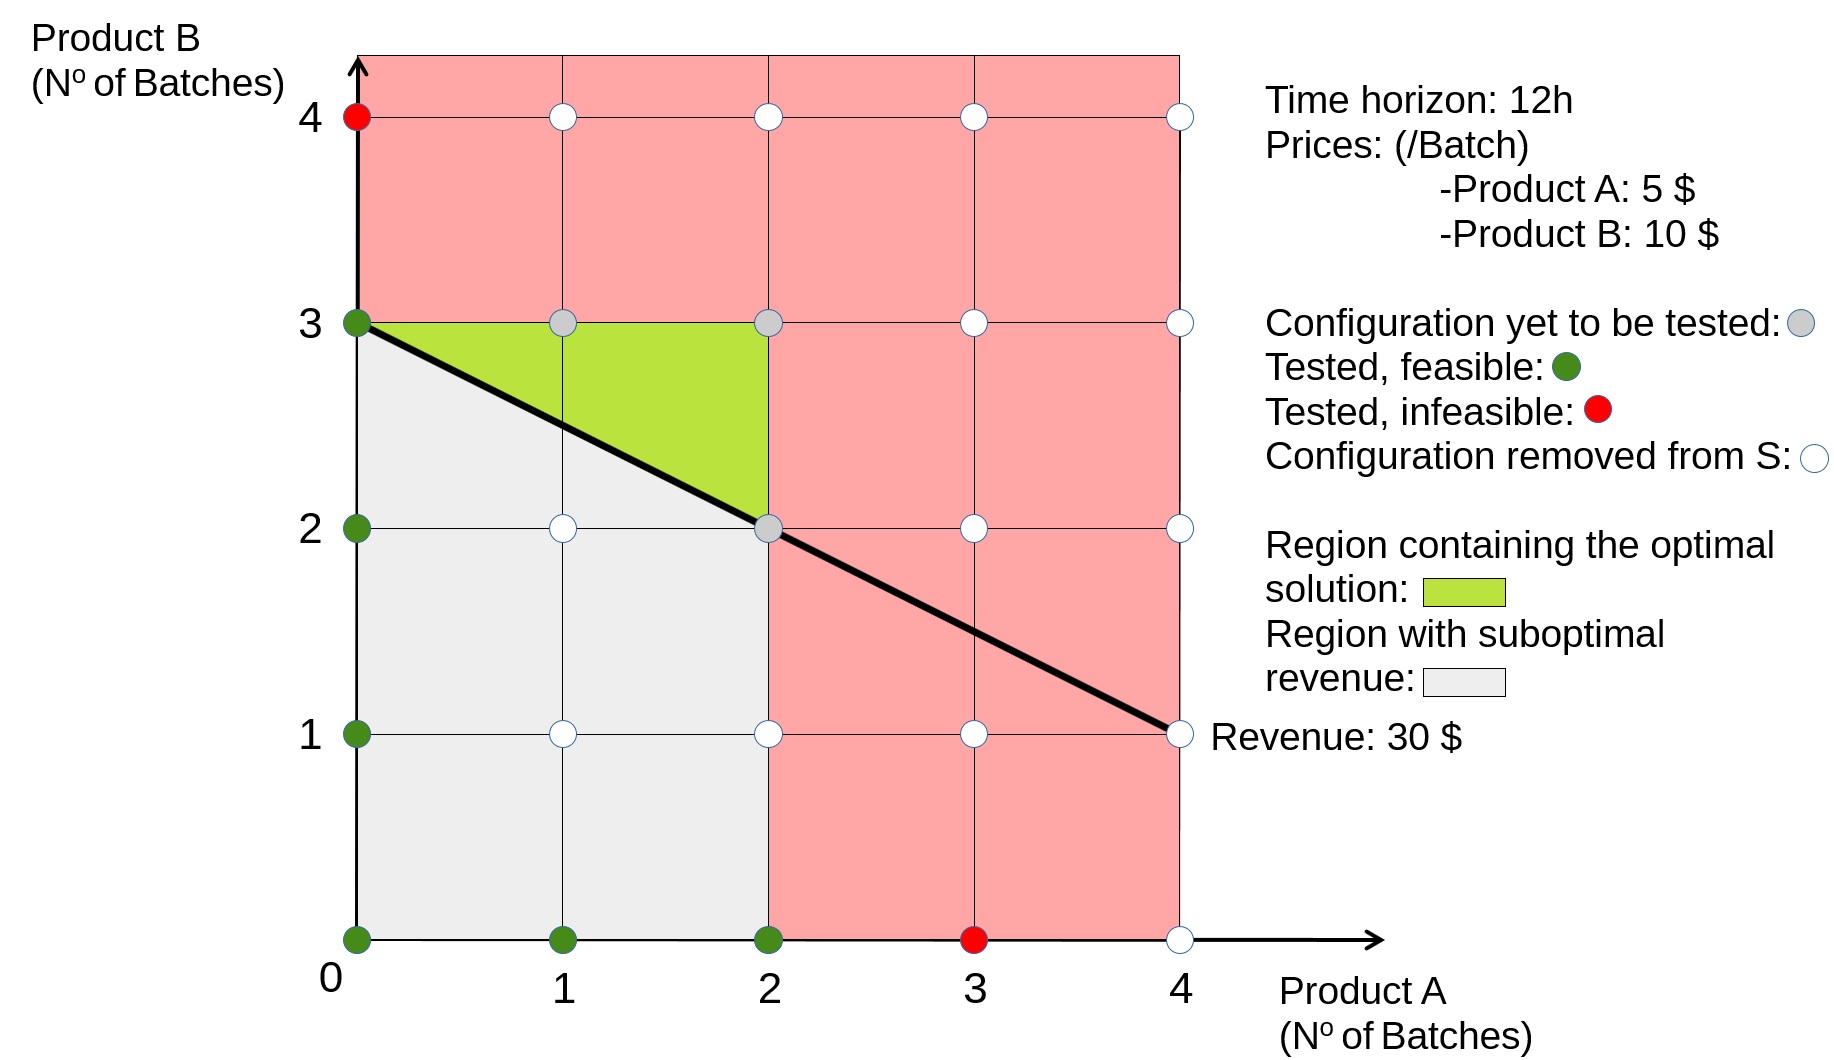
\includegraphics[scale=0.4]{revLine}
\caption{A revenue line szemléltetése}
\label{revLine}
\end{center}
\end{figure}
Jól látható, hogy jelen esetben a revenue line behúzása harmadára csökkentette az ellenőrizendő konfigurációk számát, gyorsítva ezzel az algoritmus lefutását.
Az algoritmus akkor ér véget, ha a konfigurációk halmaza kiürül, ebben az esetben ha egyetlen egy konfiguráció sem valósítható meg az adott időkorláton belül, a probléma megoldása lehetetlen az adott időhorizont alatt.
Ha található feasible megoldás, az algoritmus az optimális konfigurációt adja eredményül, megkapva ezzel a maximális profit értékét, valamint annak előállításához szükséges ütemtervet.
\section{Az S-gráf solver} \label{s-graph_framework}
Mivel munkám része a kidolgozott új módszerek implementációja az S-gráf solver programba, ezért célszerű röviden bemutatni ezen program használatát, felépítését, illetve a további munkám szempontjából fontosabb részek működését.
Ezek leírására szolgál jelen fejezet.
Az S-gráf solver program egy C++ nyelven íródott, több szálas megoldó program, mely az S-gráf keretrendszerben foglalt algoritmusok segítségével különböző ütemezési problémákat képes megoldani.
Jelenleg a NIS, UIS, UW, és LW tárolási irányelveket támogatja, valamint a következő célfüggvényekkel használható: makespan minimalizáció, throughput maximalizáció, cycle time minimalizáció.
A solver parancssorból futtatható, különböző parancssori kapcsolók teszik lehetővé a különböző funkciókhoz tartozó paraméterek beállítását.
Néhány, a throughput maximalizáláshoz fontos kapcsoló:
\begin{description}
\item[-i, \text{-{}-}input [file]] Az input fájl elérési útja, a fájl kiterjesztése .xml, vagy .ods lehet
\item[-o, \text{-{}-}output [file]] Az output fájl elérési útja, a fájl kiterjesztése lehet .txt, vagy .png attól függően, hogy szöveges, vagy grafikus megjelenítést szeretnénk eredményül kapni
\item[\text{-{}-}obj [objective function]] A célfüggvény típusa, throughput maximalizálás esetén ezen kapcsoló értéke: thmax
\item[\text{-{}-}timehor [time horizon]] A throughput maximalizáláshoz rendelkezésre álló időhorizont mérete 
\end{description}
A fentiek alapján a solver futtatására egy példa:
\begin{center}
\verb|-i input-stoch.ods -o output.png --timehor 15 --obj thmax|
\end{center}
A solver az OpenMP API-t használja párhuzamosításra, a kód lefordításához Qt5 szükséges, feltétel továbbá a boost könyvtár telepítése is.
Ezenfelül Linux alatt történő futtatáshoz letöltendő még a Google OR-Tools könyvtár, Windows operációs rendszer esetén pedig a Visual C++ Redistributable telepítése a követelmény.
A fentiek telepítése, illetve a megfelelő könyvtárak elérési útjainak beállítása után qmake segítségével elkészíthető a make file a projekt alapján.
Ezen make fájl segítségével a make meghívja a fordítót, amely lefordítja a programot, melynek következtében létrejönnek a futtatáshoz szükséges fájlok, köztük a solver.exe (Windows esetén), mellyel immáron futtathatjuk a megoldó programot az előző példához hasonló módon.   
\subsection{A solver működése}
A szolver futtatásához szükséges parancssori kapcsolók lehetséges értékeit, és egyéb paramétereit (pl. min/max érték) leíró opciókat tartalmazza az \fileName{Arguments.cpp} fájl. 
A \className{MainSolver} osztály \methodName{getOptions} metódusa a beolvasott parancssori kapcsolók értékei alapján létrehozza a \className{SolverOptions} osztály egy példányát amely objektumtól ezután lekérdezhetőek a különféle beállítások.
Ezután a \className{MainSolver} objektum \methodName{Run} metódusa meghívja a \methodName{ReadInputFromFile} metódust, ami egy \className{RelationalProblemReader} objektum példányosítása, majd annak \methodName{ReadSGraph} metódusának meghívása után vissza kapja a recept gráfot tartalmazó \className{SGraph} objektumot.
A \className{RelationalProblemReader} osztály feladata az input fájlban található paraméterek beolvasása, parse-olása, majd a recept gráf elkészítése ezek alapján.
Az \className{SGraph} osztály egy példánya lényegében egy S-gráfot reprezentál, ez lehet recept gráf, illetve ütemezési gráf is.
Ezen osztály példányosításával, paramétereinek beállításával zajlik tehát lényegében az ütemezés.
Miután a \className{MainSolver} osztály \methodName{Run} metódusa visszakapta a recept gráfot, meghívásra kerül a \methodName{GetProblem} metódus, aminek segítségével a kapcsolók, illetve a recept gráf alapján megállapításra kerül a probléma pontos típusa, ezután a \methodName{GetSolver} metódus példányosítja a probléma típus megoldásához szűkséges solvert.
Ezen solver \methodName{Solve} metódusának meghívásával elkezdődik a probléma megoldása, melynek eredményeként megkapjuk a megoldást tartalmazó \className{TreeNode} objektumot, melyen keresztül elérhető az optimális megoldást reprezentáló ütemezési gráfot tartalmazó \className{SGraph} objektum.
Throughput maximalizálás esetén ez a solver nem más, mint a \className{ThroughputSolver} osztály egy objektuma, melynek működésének leírása a \ref{throughput_solver}. pontban található.  
Az eredmény visszakapása után a \className{MainSolver} egy \className{SolutionWriter} objektum \methodName{Write} metódusának meghívásával kiíratja az eredményt a megfelelő formátumban, legyen az szöveges fájl vagy .png formátumú Gannt diagram.
\subsection{A ThroughputSolver osztály működése} \label{throughput_solver}
A \className{ThroughputSolver} lényegében a \ref{SgraphProfitMax}. alfejezetben leírtakat valósítja meg.
Az osztály \methodName{Solve} metódusa először is megkeresi az optimális megoldást tartalmazó teret, ezt azzal éri el, hogy mind addig míg található feasible konfiguráció a tengelyek mentén, létrehoz egy újabb konfigurációt, amelyben az adott termékből gyártott batchek számát növeli.
Ehhez a \methodName{FirstFeasible} metódust használja fel, mely a \methodName{SolveBest} metódus segítségével leteszteli az adott konfiguráció feasibilitását.
Ha az adott konfiguráció megvalósítható, meghívásra kerül a \methodName{NewSolution} metódus, amely a konfiguráció alapján létrehoz egy új lehetséges megoldást reprezentáló objektumot, valamint elmenti a konfiguráció profit értékét, ha az nagyobb, mint az aktuális legjobb érték.
A \methodName{SolveBest} metódus visszaadja a \methodName{FirstFeasible} metódus számára azt a mutatót, melyen keresztül az új megoldás elérhető, ha feasible volt a konfiguráció, ha nem volt az, akkor null érték kerül visszaadásra.
Az első null érték visszakapása után a \methodName{Solve} metódus több konfigurációt már nem hoz létre az aktuális tengelyen.
Miután minden tengely mentén visszakapta az első null értéket, véget ér ez az első fázis, megtalálásra került ugyanis az optimális megoldást tartalmazó tér.
Ezután következik ezen tér bejárása, az optimális megoldás megkeresése a lehetséges megoldások között.
Erre azonban több stratégia is lehetséges, ezért a \methodName{Solve} metódus először is lekérdezi az ehhez kapcsolódó parancssori paraméterek értékét, majd ezek alapján meghívja a megfelelő bejárást végző metódust.
Ez a metódus alapértelmezett esetben a \methodName{SearchThrSolution}, mely a \ref{SgraphProfitMax}. alfejezetben már említett revenue line gyorsítási stratégiát is használja a térben való kereséshez.
A metódus lefutása után ideális esetben a \methodName{Solve} metódus számára elérhetővé válik az optimális megoldást reprezentáló objektum, mely visszaadható a \className{MainSolver} számára az eredmények kiíratása érdekében.
Abban az esetben azonban, ha egyetlen lehetséges megoldás sem található a problémára, egy exception kerül eldobásra, melyet a \className{MainSolver} megfelelően le tud kezelni, jelezni tudja a felhasználó felé a tényt, miszerint nem található megoldás a problémára.